\documentclass[a4paper]{article}

\usepackage[T1]{fontenc}
\usepackage[a4paper, top=2.5cm, bottom=2.5cm, left=3cm, right=3cm]{geometry}
\usepackage{amsmath}
\usepackage{graphicx}
\usepackage{booktabs}
\usepackage{multirow}
\usepackage{float}
\usepackage{hyperref}
\usepackage[font=small,labelfont=bf]{caption}
\usepackage[style=apa, sortcites=true, sorting=ynt]{biblatex}

\addbibresource{referencias_v2.bib}

% figures/ and images/ live next to this .tex file (symlink or copy from RECURSOS/)
\graphicspath{{./figures/}{./images/}}

\hypersetup{colorlinks=true, linkcolor=black, citecolor=black, urlcolor=black}

\title{\textbf{[DRAFT] Improvements on Community Membership Hiding\\
via a Custom Reinforcement Learning Architecture}}
\author{}
\date{\today}

\begin{document}

\maketitle

\begin{abstract}
As complex networks face increasingly advanced algorithmic analysis, the ability
to conceal specific structural affiliations has emerged as a relevant graph
algorithmic problem. Current online platforms rely on sophisticated techniques
to characterize and cluster users in order to provide more contextualized content
and services. One such approach is based on community detection algorithms applied
to large underlying graphs. In this context, users are characterized by preferences
or attributes, which can reveal information that may be considered sensitive.
Community Membership Hiding (CMH) is the problem of strategically rewiring network
topology to camouflage a target node and evade detection by clustering algorithms.
While recent Deep Reinforcement Learning (DRL) approaches have pioneered this line
of work, they often face efficacy and scalability issues on large-scale graphs.
By dissecting state-of-the-art models, we identified a critical architectural
limitation: agents evaluate the network globally without explicitly conditioning on
the target node, while relying on static embeddings that fail to capture real-time
topological changes during the rewiring process.
In this paper, we introduce a novel DRL architecture designed to overcome these
fundamental limitations. We propose an Actor-Critic system powered by Graph
Attention Networks v2 (GATv2). By leveraging a target-aware feature set that
combines static original-graph indicators with dynamically updated structural
signals, and by explicitly contextualizing the target node through a dynamic
attention mechanism, our model accurately represents the evolving graph state.
We further extend this single-agent system into a \textbf{Dual-Agent Architecture}
that specializes separate agents for edge addition and edge deletion, and introduce
a \textbf{Policy-Guided Subgraphing} heuristic that makes the framework tractable
on large graphs. Extensive experimental evaluation confirms that our architecture
significantly outperforms existing baselines, achieving high hiding success rates
with minimal structural perturbation and notable gains in computational efficiency.
\end{abstract}


% ======================================================================
\section{Introduction}
% ======================================================================

The modern science of networks has brought significant advances to our
understanding of complex systems. One of the most relevant features of graphs
representing real-world structures, ranging from social media platforms to
biological networks, is their community structure, i.e.\ the identification of
tightly connected groups of nodes, task for which there exist highly effective
algorithms \parencite{Fortunato-2010}. However, in some contexts, this
functionality inherently risks exposing individuals to privacy breaches by
inadvertently revealing sensitive affiliations, such as political leanings or
religious beliefs, based solely on their structural position.

To counter this, the concept of Community Membership Hiding (CMH) has been
proposed \parencite{bernini-2024}. The objective of CMH is to strategically
alter the structural properties of a network to prevent a specific target node
from being grouped into its original community by a detection algorithm, while
maintaining overall graph integrity and ideally treating the detection algorithm
as a ``black box'' with respect to its internal mechanics.

Recent studies have formulated this evasion tactic as a Markov Decision Process
(MDP) solved via Deep Reinforcement Learning (DRL) \parencite{bernini-2024}.
While that work demonstrated the viability of the method, it exhibits notable
performance degradation when scaled to larger graphs, and has fundamental
limitations that hinder its ability to achieve optimal performance. This work
directly develops from \parencite{bernini-2024} and treats its DRL architecture
as the primary baseline reference. Building on that foundation, we dissect its
architectural shortcomings and propose a novel, efficient RL architecture that
leverages modern Graph Neural Networks to preserve privacy while maintaining
overall graph characteristics. We compare our results against three strong
baselines: the original agent introduced in \parencite{bernini-2024}, and two
gradient-based methods ($\nabla$-CMH and $\nabla$-CMH (projected)) introduced
in \parencite{silvestri2025righthidemaskingcommunity}, which improve over the
original one while achieving better computational efficiency.

We show in Section~\ref{results} that our method consistently outperforms the
original method. Against the $\nabla$- variants, we obtain better effectiveness
at a cost of more computation time --- a trade-off to consider depending on the
use case.


% ======================================================================
\section{Community Evasion}
% ======================================================================

\subsection{The Problem}

The following definitions are borrowed from \parencite{bernini-2024}. Let
$\mathcal{G} = (V, E)$ be a graph where $V$ is the set of nodes and $E$ is the
set of edges. Given a community detection algorithm $f(\cdot)$ and a target
node $u \in V$, the algorithm assigns $u$ to an original community
$\mathcal{C}_i$.

The goal of CMH is to find a modified graph $\mathcal{G}' = (V, E')$ such that
upon re-evaluating $f(\mathcal{G}')$, the new community assigned to the target
node, denoted $\mathcal{C}_i'$, is sufficiently dissimilar to the original.
Formally, the node is considered hidden when:
\begin{equation}
  \operatorname{sim}(\mathcal{C}_i - \{u\},\; \mathcal{C}_i' - \{u\}) \leq \tau
  \label{eq:hiding}
\end{equation}
where $\tau \in [0,1]$ is a predefined hiding threshold that determines the
required divergence, and $\operatorname{sim}(\cdot,\cdot)$ is a similarity
function (we use the Sørensen-Dice coefficient, following the baseline).

To aid in hiding, modifications are restricted: the agent may only remove edges
from $u$ to nodes $v \in \mathcal{C}_i$, and add edges from $u$ to nodes
$v \notin \mathcal{C}_i$. The maximum number of modifications (edge budget) is
defined through a parameter $\beta$ as:
\[
  B = \max\!\left(1,\left\lfloor \tfrac{|E|}{|V|} \cdot \beta \right\rfloor\right)
\]

In addition to hiding success, a desired property is to maximize Normalized
Mutual Information (NMI) by introducing the smallest possible structural
perturbation. We report the \textbf{F1 score}, defined as the harmonic mean of
the Success Rate (SR) and NMI, as the main evaluation metric.

\subsection{Original Agent Architecture}

To process the graph state within the established MDP framework, the baseline
of \parencite{bernini-2024} utilizes a Graph Convolutional Network (GCN)
\parencite{kipf2017semisupervisedclassificationgraphconvolutional}. The initial
node features fed into the GCN are generated using \textit{node2vec}
\parencite{grover2016node2vecscalablefeaturelearning}, which maps each node's
structural role into a latent vector space based on the initial, unaltered
graph. The agent is constrained to act on the target node via an external
environment wrapper that masks invalid actions, artificially restricting all
rewiring to the target's neighborhood.

\begin{figure}[H]
  \centering
  \includegraphics[width=0.75\linewidth]{model_architecture_background}
  \caption{Original GCN-based agent architecture from \parencite{bernini-2024}.
    The target node is not explicitly visible to the network; it is implicitly
    enforced by the action mask in the environment wrapper.}
  \label{fig:original-arch}
\end{figure}

\subsection{Architectural Limitations of the Baseline}

Upon analyzing the baseline implementation, we identified two aspects that
motivate further exploration:

\textbf{Global evaluation without target context.} The GCN receives the entire
graph as input but lacks explicit, localized knowledge of the target node $u$.
Because standard GNNs are permutation-invariant, the policy
$\pi(a \mid s)$ produces identical outputs for any target node given the same
graph state. The environment implicitly enforces valid actions, meaning the
agent's policy evaluates the global graph structure rather than explicitly
contextualizing the specific neighborhood it must camouflage. As a consequence,
the agent tends to learn a generic rewiring strategy rather than one that adapts
to the particular target being hidden.

\textbf{Static embeddings.} The \textit{node2vec} embeddings are computed only
once on the initial graph $\mathcal{G}$. As the agent actively rewires the
network, these static embeddings cease to reflect the current topological
reality. This creates an information lag that degrades learning efficiency.


% ======================================================================
\section{Proposed Architecture: GATv2 Actor-Critic}
\label{sec:gatv2-v1}
% ======================================================================

Our approach consists of an \textbf{Actor-Critic} model with a \textbf{shared
graph encoder} based on Graph Attention Networks v2 (GATv2)
\parencite{brody2022attentivegraphattentionnetworks}, designed to keep the state
representation synchronized with the evolving topology after each rewiring
action. Instead of relying on static embeddings, we build a
\textit{target-aware} feature space that combines signals from the original
graph with signals recomputed after each modification.

The feature design is organized into two complementary groups:

\textbf{Static features} (computed once on the original graph): identify
whether a node is the \textit{target node}, whether it belongs to the
\textit{target community}, and whether it is an \textit{original neighbor} of
the target.

\textbf{Dynamic features} (updated after each rewiring action): include
\textit{normalized degree}, \textit{current neighbor status} with respect to
the target, \textit{normalized common-neighbor count}, and \textit{Jaccard
similarity} to the target.

At the core, a \textbf{shared GNN backbone} of stacked GATv2 layers encodes
node features and edge information into node embeddings
$H \in \mathbb{R}^{N \times h}$. These shared embeddings are consumed by both
heads:

The \textbf{Actor head} computes per-node logits conditioned on the target
embedding $h_t$ through the scoring function $\ell_i = f(W_1 h_i + W_2 h_t)$,
where $h_i$ is the candidate-node embedding; the target node's own logit is
masked to $-\infty$. A softmax over valid logits yields the action probability
distribution $\pi(a \mid s)$.

The \textbf{Critic head} combines an attention-pooled global graph
representation $h_G = \sum_i \alpha_i h_i$, with $\alpha_i =
\operatorname{softmax}(g(h_i))$, and the target embedding to produce a scalar
state-value estimate $V(\mathcal{G}, u)$.

The reward signal is aligned with the CMH objective: a positive terminal reward
on successful hiding, a negative terminal reward on budget exhaustion, and
step-level costs that differ for edge addition vs.\ deletion to encourage
efficient rewiring.

\begin{figure}[H]
  \centering
  \includegraphics[width=0.85\linewidth]{mermaid-diagram-ac}
  \caption{GATv2 Actor-Critic v1: full architecture overview. The backbone
    is shared; both Actor and Critic heads receive the target embedding
    $h_t$ explicitly.}
  \label{fig:ac-v1-full}
\end{figure}

\begin{figure}[H]
  \centering
  \includegraphics[width=0.85\linewidth]{mermaid-diagram-backbone}
  \caption{Shared GATv2 backbone. Multi-head attention layers process node
    features and edge attributes; output is a set of node embeddings $H$.}
  \label{fig:backbone}
\end{figure}

\begin{figure}[H]
  \centering
  \begin{minipage}[t]{0.48\linewidth}
    \centering
    \includegraphics[width=\linewidth]{mermaid-diagram-actor}
    \caption{Actor head. Logits are computed by combining each candidate
      embedding with the target embedding $h_t$.}
    \label{fig:actor-head}
  \end{minipage}
  \hfill
  \begin{minipage}[t]{0.48\linewidth}
    \centering
    \includegraphics[width=\linewidth]{mermaid-diagram-critic}
    \caption{Critic head. Attention-pooled global state is concatenated with
      $h_t$ to estimate $V(\mathcal{G}, u)$.}
    \label{fig:critic-head}
  \end{minipage}
\end{figure}


% ======================================================================
\section{Architecture Comparison: Original vs.\ GATv2}
\label{sec:comparison}
% ======================================================================

\textit{(This section provides a side-by-side visual summary of the structural
differences between the baseline architecture and the proposed GATv2
Actor-Critic. Intended as a quick reference for readers familiar with the
original paper.)}

The key differences are summarized in Table~\ref{tab:arch-diff}.

\begin{table}[H]
\centering
\begin{tabular}{lll}
\toprule
\textbf{Aspect} & \textbf{Original (Bernini et al.)} & \textbf{GATv2 Actor-Critic (ours)} \\
\midrule
Graph encoder      & GCN (fixed weights) & GATv2 (dynamic attention) \\
Node features      & Static node2vec     & Static + dynamic (7 features) \\
Target awareness   & None (env mask)     & Explicit $h_t$ injection \\
Edge attributes    & Not used            & Yes (edge\_attr in backbone) \\
Actor head         & Linear over GCN out & MLP conditioned on $h_t$ \\
Critic head        & None (REINFORCE)    & Attention pooling + $h_t$ \\
Scalability        & Degrades on large graphs & Policy-Guided Subgraphing \\
\bottomrule
\end{tabular}
\caption{Structural comparison between the original baseline and the proposed
  GATv2 Actor-Critic architecture.}
\label{tab:arch-diff}
\end{table}

\begin{figure}[H]
  \centering
  \begin{minipage}[t]{0.45\linewidth}
    \centering
    \includegraphics[width=\linewidth]{model_architecture_background}
    \caption*{\textbf{Original.} The target node is not seen by the
      network; the action mask is applied externally.}
  \end{minipage}
  \hfill
  \begin{minipage}[t]{0.45\linewidth}
    \centering
    \includegraphics[width=\linewidth]{mermaid-diagram-ac}
    \caption*{\textbf{Ours (v1).} The target embedding $h_t$ is
      injected into both Actor and Critic, enabling target-specific
      decision-making.}
  \end{minipage}
  \caption{Side-by-side architecture comparison. The principal structural
    change is explicit target-node conditioning throughout the forward pass.}
  \label{fig:arch-compare}
\end{figure}


% ======================================================================
\section{Dual-Agent GATv2 Actor-Critic}
\label{sec:dual-agent}
% ======================================================================

To further improve performance---particularly NMI preservation and
scalability on large graphs---we extend the single-agent design into a
\textbf{Dual-Agent Architecture} that decomposes the rewiring task into
two specialized sub-problems.

\subsection{Agent Specialization}

The rewiring task involves two structurally distinct decisions: which
intra-community edges to sever, and which inter-community edges to form. A
single agent must learn both simultaneously, which may limit its effectiveness
on each. We split this into two dedicated agents:

\textbf{Adder Agent:} trained exclusively to identify and create beneficial
inter-community edges from $u$ to nodes outside $\mathcal{C}_i$.

\textbf{Deleter Agent:} trained exclusively to identify and remove critical
intra-community edges from $u$ to nodes inside $\mathcal{C}_i$.

Both agents share the same GATv2-based backbone design (same feature space,
same encoder architecture), but maintain independent Actor and Critic heads,
each trained on their respective action subspace.

\subsection{Action-Selection via Critic Comparison}

At each timestep, both agents are queried in parallel. The agent selected to
act is the one whose Critic reports the higher expected state value:
\[
  \text{act} = \arg\max_{a \in \{\text{add}, \text{del}\}} V_a(\mathcal{G}, u)
\]
This value-based selection allows the architecture to adaptively switch between
addition and deletion depending on which is more beneficial given the current
graph state, without any hand-crafted switching rule. The Critics, originally
introduced to stabilize training via advantage estimation, thus serve a
second role as a routing mechanism.

\begin{figure}[H]
  \centering
  
\includegraphics[width=0.85\linewidth]{mermaid-dual-agent}
  \caption{Dual-Agent GATv2 Actor-Critic. Each agent has independent Actor
    and Critic heads but shares the same backbone design. At each step the
    agent with the higher Critic value is selected to act.}
  \label{fig:dual-agent}
\end{figure}

\subsection{Scaling via Policy-Guided Subgraphing}

A key bottleneck on large graphs is the cost of recomputing dynamic features
(Common Neighbors, Jaccard Similarity) for all nodes after every action, which
grows with $|V|$ and $|E|$. We address this with a \textbf{Policy-Guided
Subgraphing} heuristic, which proceeds in five stages:

\begin{enumerate}
  \item Both Actor networks perform a single forward pass on the full graph to
    produce raw logits (no feature updates at this stage).
  \item The top-$k$ nodes preferred by each agent are identified from the logits.
  \item Those node selections are expanded to the full communities of the
    retained nodes.
  \item A reduced subgraph is constructed containing only those communities
    together with the target node.
  \item All subsequent dynamic feature updates and rewiring actions are executed
    inside this reduced subgraph.
\end{enumerate}

This heuristic trades a small, controllable reduction in F1 score for a
substantial decrease in per-step computation, making previously intractable
large graphs feasible. We compare it against a simpler \textit{k-neighborhood}
baseline (extracting the $k$-hop ego-graph of $u$), which tends to miss distant
bridge nodes that would be ideal for inter-community connections.


% ======================================================================
\section{Results}
\label{results}
% ======================================================================

We report results using the F1 score (harmonic mean of SR and NMI), following
the standard CMH evaluation protocol \parencite{bernini-2024}. Experiments were
run on an AWS EC2 \texttt{g4dn.xlarge} instance (4 Intel Xeon vCPUs, 16 GiB
RAM, NVIDIA T4 GPU) over five benchmark datasets of varying size and density.
We swept $\tau \in \{0.3, 0.5, 0.8\}$ and $\beta \in \{0.5, 1.0, 2.0\}$.

\subsection{GATv2 Actor-Critic v1 vs.\ Baselines}

To evaluate the robustness of our approach to the hiding threshold ($\tau$) and
edge budget ($\beta$), we performed a full parameter sweep and compared success
rates against the original agent. Table~\ref{tab:success_rate_comparison} shows
the overall consistency of the results across configurations.

\begin{table}[H]
\centering
\begin{tabular}{llcc}
\toprule
\textbf{$\beta$} & \textbf{$\tau$} & \textbf{GATv2 v1 (ours)} & \textbf{Original} \\
\midrule
\multirow{3}{*}{0.5} & 0.3 & 61.67 & 41.67 \\
                     & 0.5 & 70.21 & 38.22 \\
                     & 0.8 & 79.38 & 62.67 \\
\midrule
\multirow{3}{*}{1.0} & 0.3 & 79.17 & 61.67 \\
                     & 0.5 & 91.78 & 58.44 \\
                     & 0.8 & 96.25 & 90.00 \\
\midrule
\multirow{3}{*}{2.0} & 0.3 & 82.08 & 77.67 \\
                     & 0.5 & 98.75 & 74.67 \\
                     & 0.8 & 99.17 & 96.33 \\
\bottomrule
\end{tabular}
\caption{Success rates (\%) for GATv2 v1 vs.\ original agent, averaged
         across datasets and community detection algorithms.}
\label{tab:success_rate_comparison}
\end{table}

The proposed agent demonstrates a substantial and consistent improvement across
all tested configurations. Stricter hiding constraints (lower $\tau$) naturally
increase difficulty, but our architecture maintains a robust performance gap
over the baseline. With moderate-to-high budget allowances ($\beta \geq 1.0$)
our model achieves near-perfect success rates, whereas the original agent's
performance prematurely plateaus. Importantly, the proposed architecture
maintains consistent behavior across the full parameter grid, without
overfitting to a single scenario.

Figure~\ref{fig:tradeoff-f1-time} summarizes the F1/time tradeoff for a
representative configuration ($\tau=0.5$, $\beta=1$) across all datasets.
While the gradient-based $\nabla$-CMH methods achieve better computational
efficiency, they sacrifice F1 score; our architecture occupies the high-F1
end of the tradeoff.

\begin{figure}[H]
  \centering
  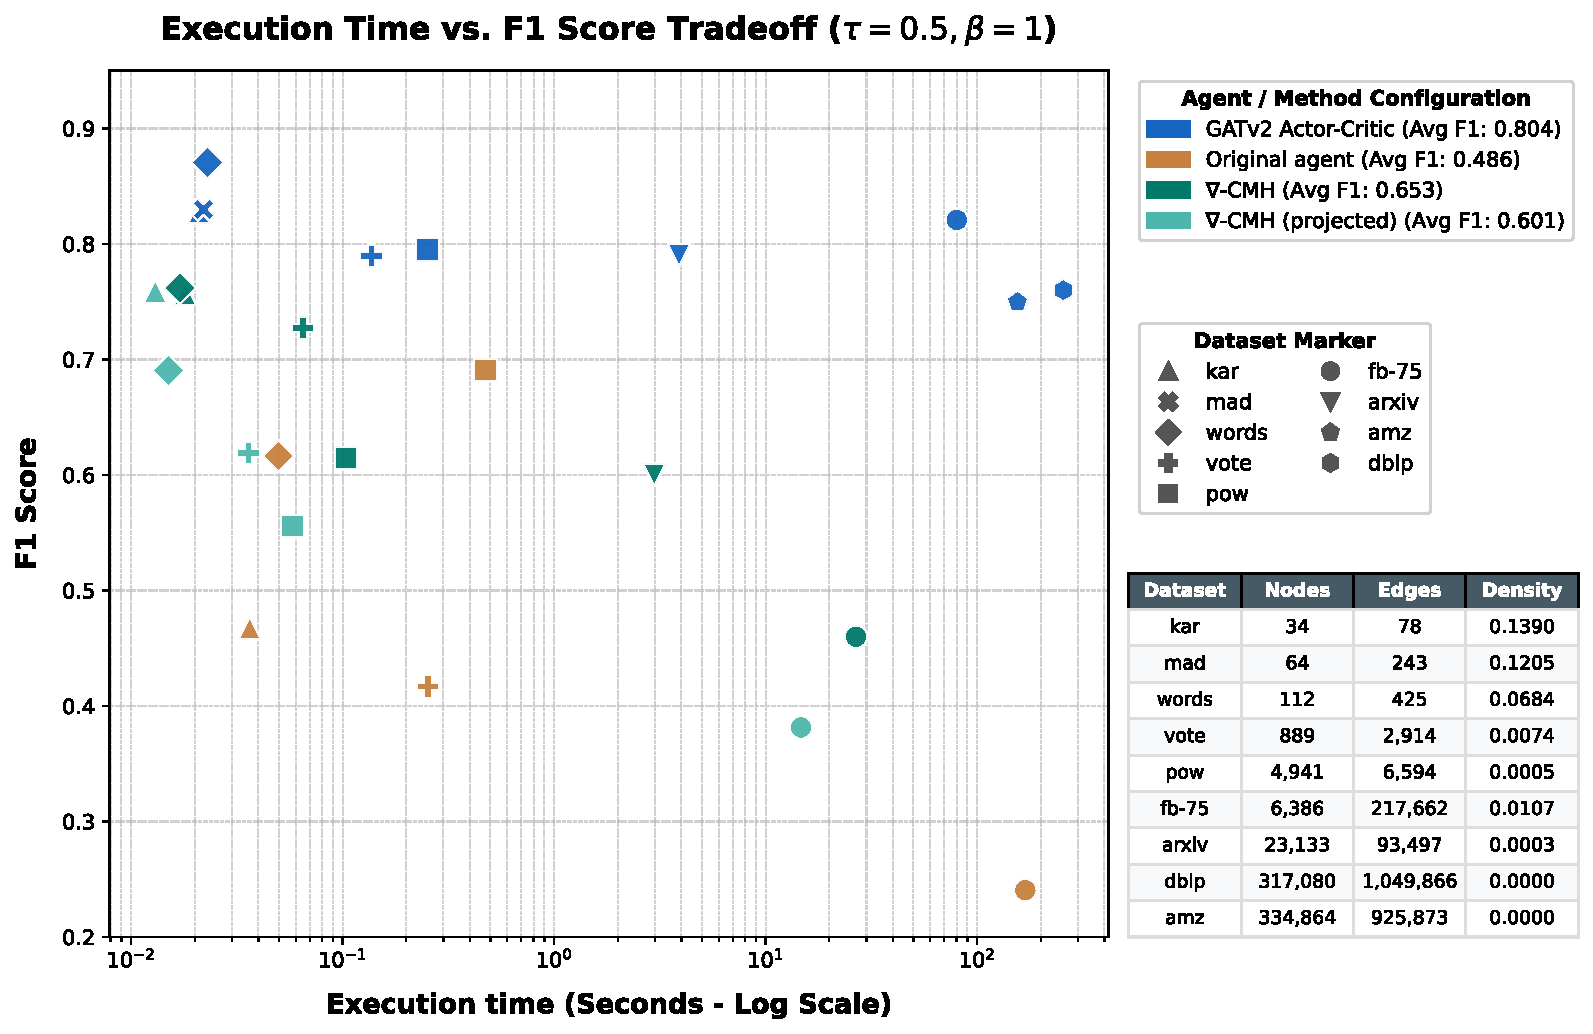
\includegraphics[width=0.92\linewidth]{tradeoff_plot}
  \caption{F1 score vs.\ execution time ($\tau=0.5,\ \beta=1$).
           Time axis in logarithmic scale. Each point is one method on one
           dataset/algorithm combination.}
  \label{fig:tradeoff-f1-time}
\end{figure}

Figure~\ref{fig:sr-nmi-all} shows per-dataset SR and NMI breakdowns for the
three community detection algorithms evaluated.

\begin{figure}[H]
  \centering
  
\includegraphics[width=0.92\linewidth]{F1_allDatasets_evaluation_node_hiding_greedy_multiAgents}
  \caption{F1 score per dataset --- Greedy Modularity community detection
    ($\tau=0.5,\ \beta=1$).}
  \label{fig:f1-greedy}
\end{figure}

\begin{figure}[H]
  \centering
  
\includegraphics[width=0.92\linewidth]{F1_allDatasets_evaluation_node_hiding_louvain_multiAgents}
  \caption{F1 score per dataset --- Louvain community detection
    ($\tau=0.5,\ \beta=1$).}
  \label{fig:f1-louvain}
\end{figure}

\begin{figure}[H]
  \centering
  
\includegraphics[width=0.92\linewidth]{F1_allDatasets_evaluation_node_hiding_walktrap_multiAgents}
  \caption{F1 score per dataset --- Walktrap community detection
    ($\tau=0.5,\ \beta=1$).}
  \label{fig:f1-walktrap}
\end{figure}
\label{fig:sr-nmi-all}

\subsection{Dual-Agent Results}

\textit{(This section will report the final empirical comparison for the
dual-agent variant once the full evaluation sweep is complete.)}

\begin{figure}[H]
  \centering
  \fbox{\parbox[c][4cm][c]{0.85\linewidth}{\centering
    \textbf{[Placeholder]} Dual-Agent F1 results across datasets and
    community detection algorithms ($\tau=0.5,\ \beta=1$).}}
  \caption{Dual-Agent F1 results. \textit{(Figure to be included.)}}
  \label{fig:dual-results}
\end{figure}

\begin{figure}[H]
  \centering
  \fbox{\parbox[c][4cm][c]{0.85\linewidth}{\centering
    \textbf{[Placeholder]} Effect of Policy-Guided Subgraphing on
    execution time and F1 score on large graphs.}}
  \caption{Policy-Guided Subgraphing: scaling results.
    \textit{(Figure to be included.)}}
  \label{fig:subgraph-scaling}
\end{figure}


% ======================================================================
\section{Parameter Sweep}
\label{sec:sweep}
% ======================================================================

\textit{(This section presents a visual summary of how F1 score varies jointly
with the hiding threshold $\tau$ and the rewiring budget $\beta$. Each 3D
surface corresponds to one of the three community detection algorithms
evaluated: Greedy Modularity, Louvain, and Walktrap. Values are averaged across
datasets. Figures to be included once the full sweep is finalized.)}

To better understand the joint sensitivity of the proposed architecture to
$\tau$ and $\beta$, we run a full grid sweep over
$\tau \in \{0.3, 0.5, 0.8\}$ and $\beta \in \{0.5, 1.0, 2.0\}$ for each
community detection algorithm. The resulting F1 surfaces are shown in
Figures~\ref{fig:sweep-greedy}--\ref{fig:sweep-walktrap}.

\begin{figure}[H]
  \centering
  \includegraphics[width=0.85\linewidth]{sweep_greedy}
  \caption{F1 score surface over $(\tau, \beta)$ for the \textbf{Greedy
    Modularity} community detection algorithm.
    \textit{(Figure to be included.)}}
  \label{fig:sweep-greedy}
\end{figure}

\begin{figure}[H]
  \centering
  \includegraphics[width=0.85\linewidth]{sweep_louvain}
  \caption{F1 score surface over $(\tau, \beta)$ for the \textbf{Louvain}
    community detection algorithm.
    \textit{(Figure to be included.)}}
  \label{fig:sweep-louvain}
\end{figure}

\begin{figure}[H]
  \centering
  \includegraphics[width=0.85\linewidth]{sweep_walktrap}
  \caption{F1 score surface over $(\tau, \beta)$ for the \textbf{Walktrap}
    community detection algorithm.
    \textit{(Figure to be included.)}}
  \label{fig:sweep-walktrap}
\end{figure}

In general, larger $\beta$ (more budget) and larger $\tau$ (softer hiding
criterion) make the task easier, and the F1 surface reflects this monotone
trend. The most interesting regime is around intermediate values
($\tau \approx 0.5$, $\beta \approx 1.0$), where the proposed architecture
shows the largest relative improvement over baselines.
\textit{(Exact numbers to be added once dual-agent sweep is complete.)}


% ======================================================================
\section{Conclusions and Further Work}
% ======================================================================

We show that architectural alignment between representation, decision, and
reward is central to scalable CMH. By combining target-aware feature
construction, a shared GATv2 encoder, and coordinated Actor-Critic heads, the
proposed method improves the tradeoff between hiding success and structural
preservation. The Dual-Agent extension further decomposes the rewiring task
into specialized sub-problems, and the Policy-Guided Subgraphing heuristic
extends the framework to large graphs that were previously intractable.

Beyond the specific benchmark gains, the results suggest that RL-based graph
evasion benefits substantially from feature designs that remain synchronized
with graph evolution during rewiring. This perspective opens a practical path
toward extending the framework to broader hiding scenarios. In the near future,
we plan to extend this framework to overlapping community detection scenarios
and to multi-node hiding settings.

\textit{(Quantitative conclusions for the dual-agent variant to be added.)}

\printbibliography[heading=bibintoc,title={References}]

\end{document}
